\documentclass[12pt, 
hyperref={colorlinks=true, linkcolor=blue, urlcolor=cyan}]{beamer}
\usetheme{default} 

\setbeamertemplate{navigation symbols}{} %gets rid of navigation symbols
\setbeamertemplate{footline}{} %gets rid of bottom navigation bars
\setbeamertemplate{footline}[page number]{} %use this for page numbers

\setbeamertemplate{itemize items}[circle] %round bullet points
\setlength\parskip{10pt} % white space between paragraphs

\setbeamertemplate{footline}{%
  \raisebox{5pt}{\makebox[\paperwidth]{\hfill\makebox[10pt]{\scriptsize\insertframenumber~~}}}}
  
\usepackage{wrapfig}
\usepackage{subfig}
\usepackage{setspace}
\usepackage{enumerate}
\usepackage{graphicx}
\usepackage{amsmath}
\usepackage{amsfonts}
\usepackage{amssymb}
\usepackage{amsthm}
\usepackage[UKenglish]{isodate}
\cleanlookdateon

% the preamble
\title{BIOST 311: \\ Regression Methods for the Health Sciences}
\author{Kelsey Grinde and Brian Williamson}
\institute{UW Biostatistics}
\date{3 April 2018}

\begin{document}
% title slide
\begin{frame}
\titlepage\thispagestyle{empty}
\end{frame}


\begin{frame}
\frametitle{DISCUSSION SECTION 2 }
\framesubtitle{GRAPHS AND TABLES: Interpretation, recommendations, and guidelines}

{\small

Some good references (both for the content in these slides and for general thoughts on displaying data):
{\scriptsize
\begin{itemize}
\item Tufte ER. The Visual Display of Quantitative Information. Graphics Press, Cheshire, Connecticut, 1983.
\item Wainer H. (1984) How to display data badly. American Statistician 38(2):137--147.
\item Proschan M. (2016) FDA Advisory Committees: the role of statisticians. Chance 29(3):31--40.
\item \href{https://www.biostat.wisc.edu/~kbroman/topten\_worstgraphs/}{Karl Broman's website}
\end{itemize}
}

The content in these slides is courtesy of Professor Jim Hughes (we have made minor modifications). 
}
\end{frame}

\begin{frame}
\frametitle{Graphs vs tables}
Graphs:
\begin{itemize}
\item Good for showing \textcolor{blue}{qualitative trends} (e.g., increasing)
\item[]
\item Good for displaying \textcolor{blue}{large amounts} of data
\end{itemize}

Tables:
\begin{itemize}
\item Good for showing \textcolor{green}{exact values}
\item[]
\item Good for displaying \textcolor{green}{small amounts} of data
\end{itemize}

Today, we'll cover guidelines for good graphics and tables!
\end{frame}

\begin{frame}
\frametitle{Graphical integrity: representing numbers}

The representation of numbers, 

\textcolor{blue}{as physically measured} on the surface of the graphic, 

should be \textcolor{green}{directly proportional} to the numerical quantities represented.

\end{frame}

\begin{frame}
\frametitle{Graphical integrity: representing numbers}
\vspace{0.1cm}
What's \textcolor{red}{wrong} with this graph?

\centering
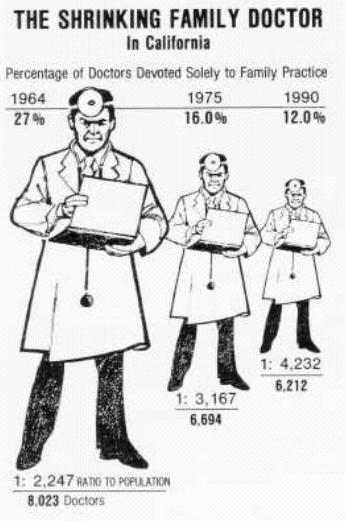
\includegraphics[height = 0.85\textheight]{{figs/proportional_1}.png}
\end{frame}


\begin{frame}
\frametitle{Graphical integrity: representing numbers}
Guess the percentages (hint: they sum to 100\%):

\centering
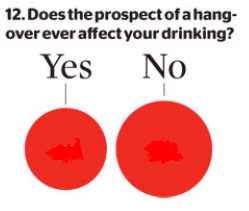
\includegraphics[width = 0.6\textwidth]{{figs/proportional_2}.png}
\end{frame}

\begin{frame}
\frametitle{Graphical integrity: representing numbers}
\centering
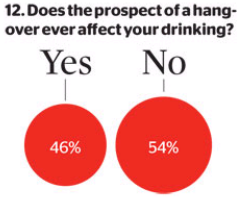
\includegraphics[width= 0.6\textwidth]{{figs/proportional_3.png}}
\end{frame}

\begin{frame}
\frametitle{Graphical integrity: reference points}

Provide \textcolor{blue}{an appropriate reference point},

 \textcolor{green}{spacing}, 
 
 and \textcolor{cyan}{labeling} for axes.

\end{frame}


\begin{frame}
\frametitle{Graphical integrity: reference points}

\begin{center}
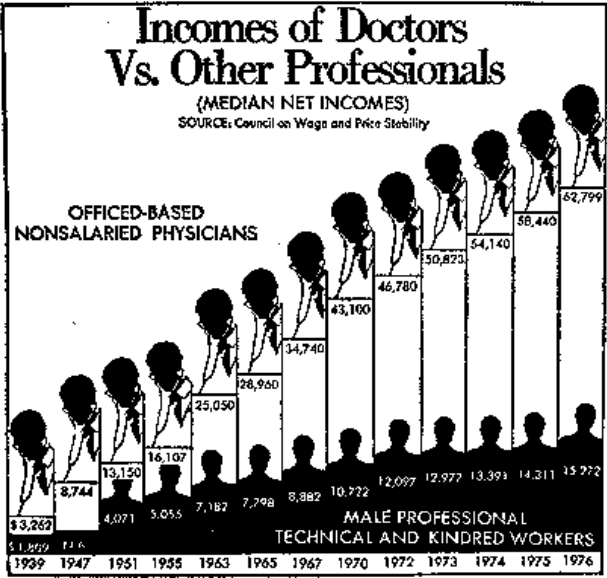
\includegraphics[width=0.8\textwidth]{{figs/reference_1.png}}
\end{center}

\end{frame}


\begin{frame}
\frametitle{Graphical integrity: reference points}
The previous plot, with a \textcolor{blue}{correctly scaled} $x$-axis:

\centering
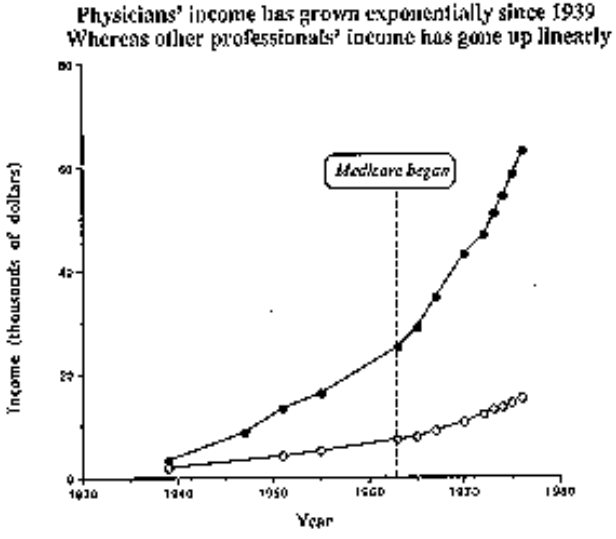
\includegraphics[width=0.8\textwidth]{{figs/reference_2}.png}
\end{frame}


\begin{frame}
\frametitle{Graphical integrity: reference points}

\centering
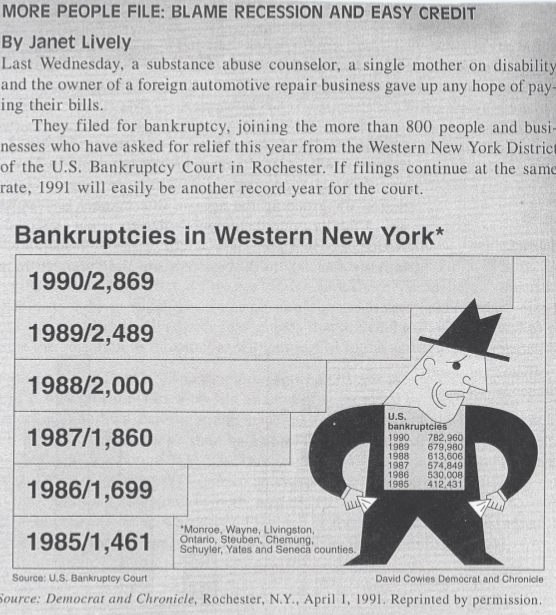
\includegraphics[height=0.9\textheight]{{figs/reference_3}.png}

\vspace{-0.5cm}
{\scriptsize From: Johnson R. Just the Essentials of Statistics. Duxbury Press, 1995.}
\end{frame}


\begin{frame}
\frametitle{Graphical integrity: reference points}
What's the \textcolor{blue}{message}?

\centering
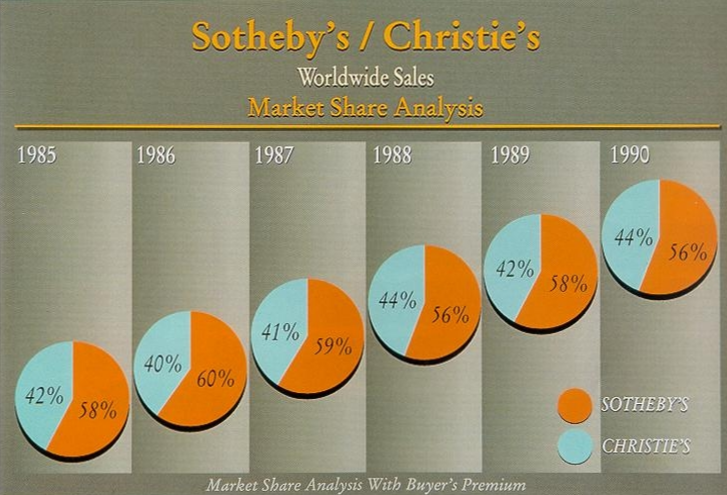
\includegraphics[width=0.9\textwidth]{{figs/reference_4}.png}
\end{frame}


\begin{frame}
\frametitle{Graphical integrity: reference points}
A more reasonable presentation:

\centering
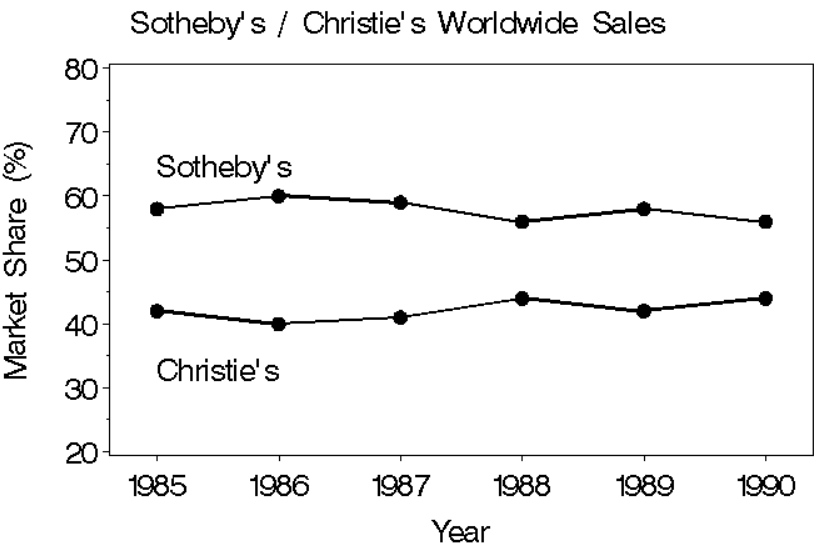
\includegraphics[width=0.9\textwidth]{{figs/reference_5}.png}
\end{frame}


\begin{frame}
\frametitle{Graphical integrity: reference points}

\centering
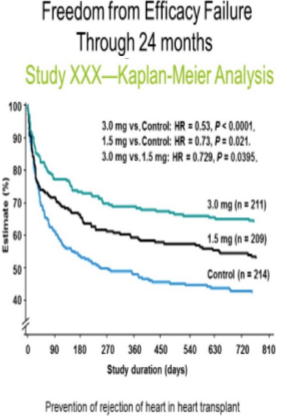
\includegraphics[height = 0.9\textheight]{{figs/reference_6}.png}
\end{frame}


\begin{frame}
\frametitle{Graphical integrity: reference points}

\centering
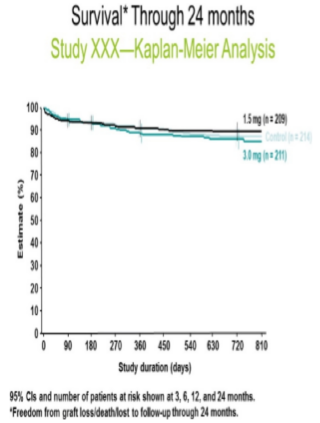
\includegraphics[height = 0.9\textheight]{{figs/reference_7}.png}
\end{frame}


\begin{frame}
\frametitle{Graphical integrity: context}

\textcolor{red}{Do not quote data out of context}.
\end{frame}


\begin{frame}
\frametitle{Graphical integrity: context}

\centering
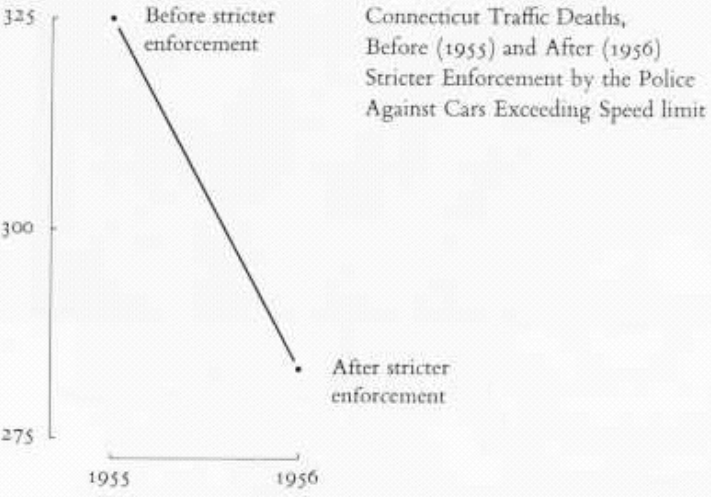
\includegraphics[width=0.9\textwidth]{{figs/context_1}.png}
\end{frame}


\begin{frame}
\frametitle{Graphical integrity: context}

\centering
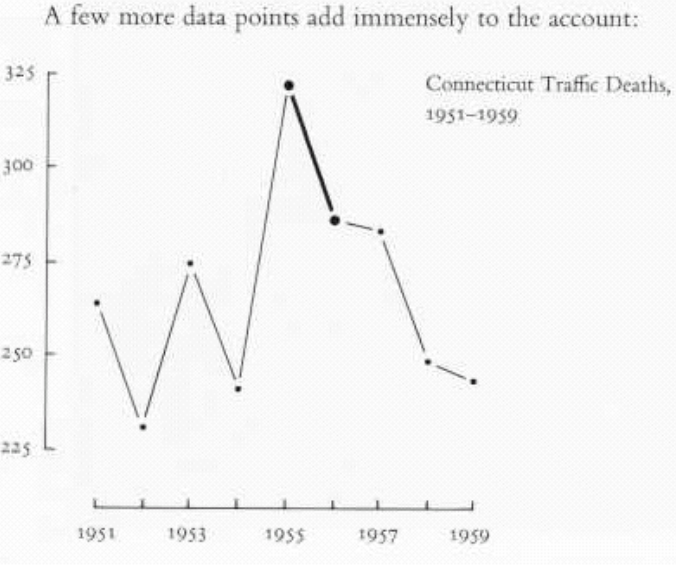
\includegraphics[width=0.9\textwidth]{{figs/context_2}.png}
\end{frame}


\begin{frame}
\frametitle{Graphical integrity: focus on the data}

Focus on the data, 

\textcolor{red}{not the design}, 

and maximize the data:ink ratio. 

\end{frame}


\begin{frame}
\frametitle{Graphical integrity: focus on the data}

\centering
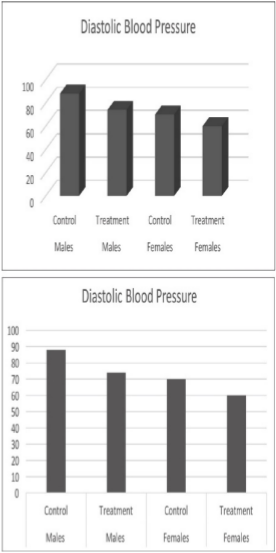
\includegraphics[height=0.9\textheight]{{figs/ink_1}.png}
\end{frame}


\begin{frame}
\frametitle{Graphical integrity: focus on the data}

How much information is displayed in this graph?

\centering
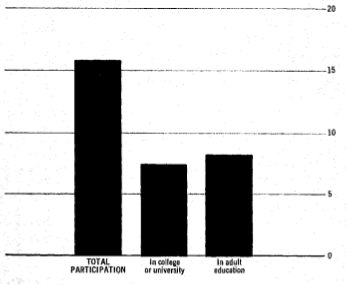
\includegraphics[height=0.85\textheight]{{figs/ink_2}.png}

\end{frame}


\begin{frame}
\frametitle{Graphical integrity: labeling}

Use \textcolor{blue}{clear, detailed, and thorough labeling} to \textcolor{red}{defeat graphical distortion and ambiguity}. 

\textcolor{green}{Write out explanations} of the data on the graphic itself. \textcolor{cyan}{Label important events} in the data.

Captions should be \textcolor{blue}{self-contained}, so that the reader does not have to refer back to the text to understand the graphic.
\end{frame}


\begin{frame}
\frametitle{Graphical integrity: labeling}

\hspace*{-1cm}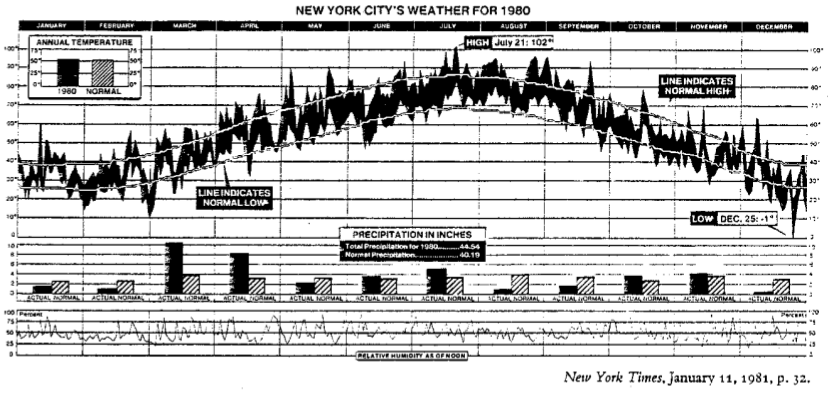
\includegraphics[width=1.2\textwidth]{{figs/good_1}.png}
\end{frame}

%%%%%%%%%%%%%%%%%%%%%%%%%%%%%%%%%%%%%%
%% THIS BIT MAY BE REMOVED
%%%%%%%%%%%%%%%%%%%%%%%%%%%%%%%%%%%%%%
%\begin{frame}
%\frametitle{Pie charts: the good}
%
%\end{frame}
%
%
%\begin{frame}
%\frametitle{Pie charts: the bad}
%
%\end{frame}
%
%
%\begin{frame}
%\frametitle{Pie charts: the ugly}
%
%\end{frame}

%%%%%%%%%%%%%%%%%%%%%%%%%%%%%%%%%%%%%%
%% THIS BIT IS IMPORTANT AGAIN
%%%%%%%%%%%%%%%%%%%%%%%%%%%%%%%%%%%%%%

\begin{frame}
\frametitle{Graphical integrity: summary}
Remember that graphics should \textcolor{blue}{support your statistical analyses}.

Components of good graphics:
\begin{itemize}
\item Figures should be \textcolor{blue}{proportional} to the numerical quantities represented
\item[]
\item Include \textcolor{blue}{reference points}, \textcolor{blue}{spacing} and \textcolor{blue}{labeling} for axes
\item[]
\item \textcolor{red}{Do not quote the data out of context}
\item[]
\item Focus on the \textcolor{blue}{data}, \textcolor{red}{not the design}
\item[]
\item \textcolor{blue}{Clear}, \textcolor{blue}{detailed}, and \textcolor{blue}{thorough} labeling
\end{itemize}
\end{frame}


%\begin{frame}
%\frametitle{Graphical integrity: summary}
%
%\hspace*{-1cm}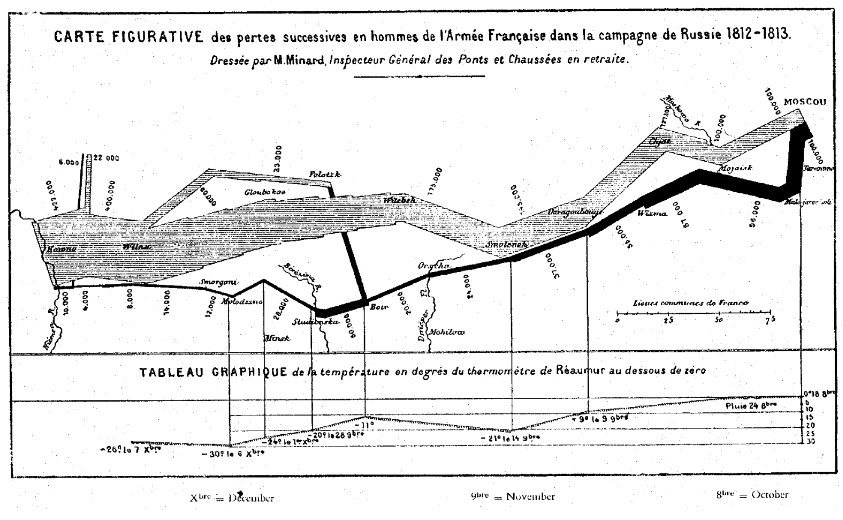
\includegraphics[width=1.15\textwidth]{{figs/good_2}.png}
%\end{frame}


\begin{frame}
\frametitle{Guidelines for tables (Ehrenberg, 1977)}
\begin{itemize}
\item Give \textcolor{blue}{marginal averages} to provide a visual focus
\item[]
\item Order rows/columns by marginal averages or other \textcolor{green}{measure of size}
\item[]
\item Put groups to be compared in rows (so that scanning down columns yields comparisons)
\item[]
\item Round to 2 effective digits
\item[]
\item Use layout to facilitate comparisons
\item[]
\item Give \textcolor{blue}{brief verbal summaries} to lead reader to patterns and exceptions
\item[]
\item Clearly label rows/columns, give units, title
\end{itemize}
\end{frame}


\begin{frame}
\frametitle{Tables: example }
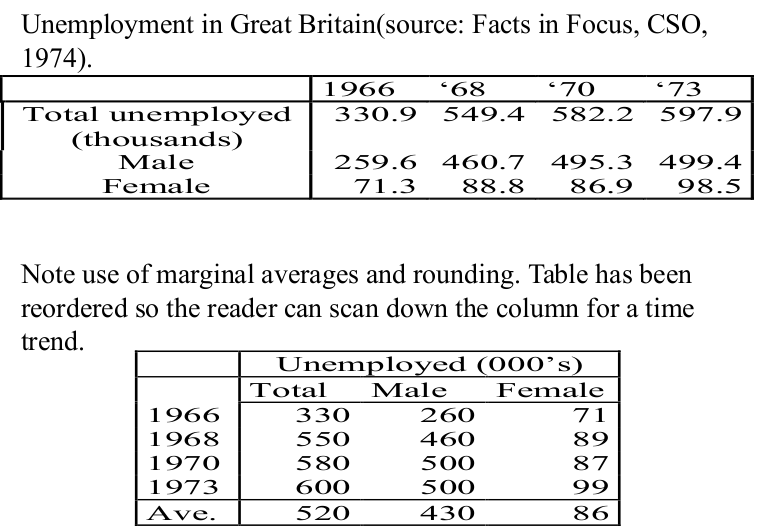
\includegraphics[width=1\textwidth]{{figs/tables_1}.png}
\end{frame}


%\begin{frame}
%\frametitle{Tables: example 2}
%\centering
%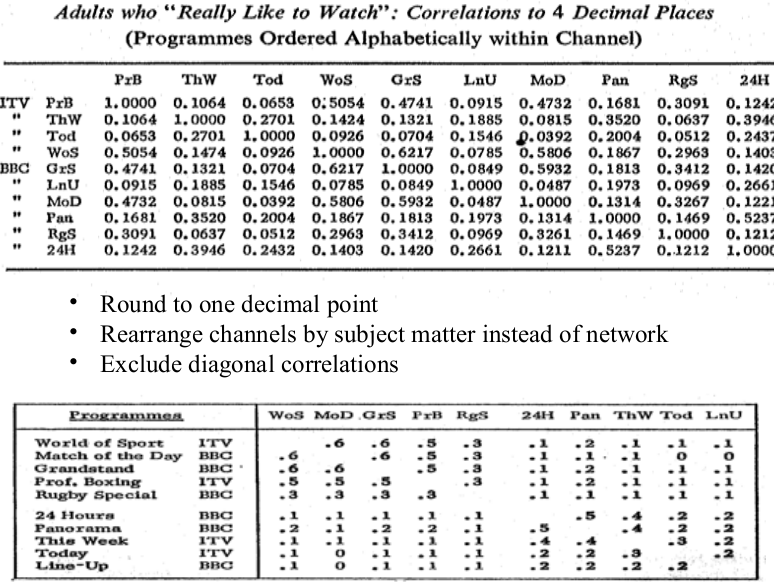
\includegraphics[width=1\textwidth]{{figs/tables_2}.png}
%\end{frame}


\end{document}
